\documentclass[letterpaper,12pt]{article}
\usepackage[utf8]{inputenc}
\usepackage{fullpage}
\usepackage{courier}
\usepackage[margin=0.75in]{geometry}
\usepackage{listings}
\usepackage{color}
\usepackage{graphicx}
\usepackage[width=5in]{caption}
\usepackage{hyphenat}
\usepackage[section]{placeins}

% Format a sectionless paragraph
\newcommand*\unparagraph{
	\par
	\nopagebreak
	\vskip3.25ex plus1ex minus.2ex
	\noindent
}

% define extra colors
\definecolor{dkgreen}{rgb}{0,0.6,0}
\definecolor{purple}{RGB}{159,0,197}

% define the code listing format
\lstset{
	language=C++,
	basicstyle=\footnotesize\ttfamily,
	backgroundcolor=\color{white},
	showspaces=false,
	showstringspaces=false,
	frame=none,
	tabsize=3,
	keywordstyle=\color{purple},
	commentstyle=\color{dkgreen},
	stringstyle=\color{blue},
	escapeinside={\%*}{*)}
}

% define the title/header
\title{\Large CS 1428 Honors\\Lab 0} 
\author{Jared Wallace}
\date{}

\begin{document}

\maketitle

\vspace{30mm}

\section*{Questions}
\begin{enumerate}
    \item (10 pts) What environment do we use to develop and compile our C++ programs? What is the name of the compiler our environment uses?
    \vspace*{40mm}
    \item (25 pts) Using the Code::Blocks IDE, (or the text editor of your choice) write a very
                   simple program. Requirements:
                   \begin{enumerate}
                        \item It must output your name, today’s date, and your lecture/section number.
                        \item Name the source file lab00h.cpp.
                        \item Make sure to include the standard header as discussed in class
                        \item Compile and run the program.
                        \item Print and attach the source code to this work sheet.
                        \item Upload the source to the homework upload.
                    \end{enumerate}
    \item (10 pts) What is an algorithm?
    \vspace*{40mm}
    \item (10 pts) What is Computer Science?
    \vspace*{40mm}
    \item (10 pts) What are some expressions? Make up 6 different, valid, C++ expressions.
    \vspace*{40mm}
    \item (10 pts) What are the steps to start writing a program in Code::Blocks? 
    \vspace*{40mm}
    \item (10 pts) What is the difference between assembly and machine code?
    \vspace*{40mm}
    \item (15 pts) Label the diagram
\end{enumerate}
\begin{figure}[h!]
    \centering
    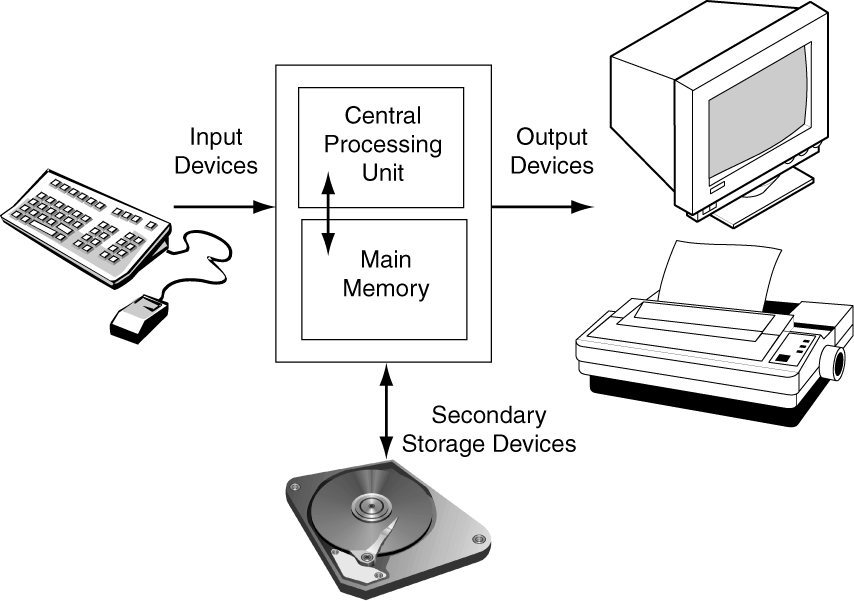
\includegraphics[width=5in]{graphic.png}
\end{figure}

\section*{Deliverables}
The source code you wrote (lab0h.cpp) and the answers to the questions.

% Comic at the bottom
\begin{figure}[ht!]
	\centering
	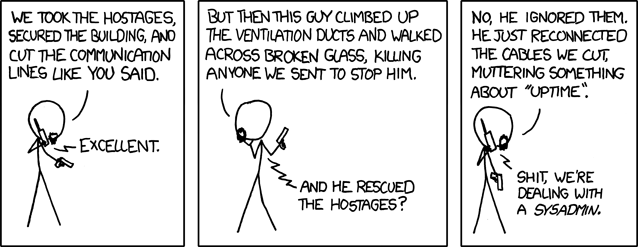
\includegraphics[width=5in]{devotion_to_duty.png}
	\caption*{The weird sense of duty really good sysadmins have can border on the sociopathic, 
		but it's nice to know that it stands between the forces of darkness and your cat blog's servers.}
\end{figure}
\end{document}
